\section{第1讲\quad 数值计算}

\item {
    【乘法分配律】
    $(200+2)\times 5 + 5020$
    \vspace{1cm}
    % 改. 2025
}

\item {
    【乘法分配律】
    $7\times 19 + 3\times 13\times 41 + 13\times 19$
    \vspace{1cm}
    % 改. 2021;迎春杯四年级真题.pdf
}

\item {
    【乘法分配律】
    $(18\times 23 - 24\times 17)\div 3 + 5$
    \vspace{1cm}
}

\item {
    【乘法分配律】
    $(11\times 24 - 23\times 9)\div 3 + 3$
    \vspace{1cm}
}

\item {
    【乘法凑十】
    $12\times 25 + 16\times 15$
    \vspace{1cm}
}

\item {
    【乘法凑十】
    $5\times 432\times 1 - 98 - 7\times 6$
    \vspace{1cm}
    %  2020数学花园探秘笔试小中决赛D卷.doc
}

\item {
    【加法凑十】
    $1+3+4+6+7+9+10 + 12$
    \vspace{1cm}
}

\item {
    【乘法凑十】
    $210\times 6 - 52\times 5$
    \vspace{1cm}
}

\item {
    【尾同头合十】
    $5000- 22\times 82$  
    \vspace{1cm}
}

\item {
    【乘法分配律】
    $67\times 67 - 34\times 34 + 67 + 34$
    \vspace{1cm}
    % 2017年“迎春杯”数学花园探秘科普活动试卷(小中组决赛a卷).doc
}

\item {
    【等差数列求和公式】
    $(1+3+5+\cdots + 89) - (1+2+3+\cdots + 63)$  
    \vspace{1cm}
}

\item {
    【数列】
    数列$1, 1,2,3,5,8\cdots$从第二项起每一项都等于它前面两项之和,这个数列成为斐波那契数列.其中每一项都叫做斐波那契数.可以证明“任意正整数n都可以成若干个不同的斐波那契数之和”,那么把100表示成若干个不同的斐波那契数之和有\underline{\hbox to 20mm{}}种表示方法.(只是交换加数的顺序算作同一种)  
    \vspace{1cm}
    % 2016年“迎春杯”数学花园探秘初赛试卷(四年级b卷).doc
}

\item {
    【立方和公式】
    $3^3 + 4^3 + 5^3 + 6^3 + 7^3 + 8^3 + 9^3$
    \vspace{1cm}
}

\item {
    【数值计算】
    $99\times 10101\times 111\times 1001001$的末5位数字是多少?
    \vspace{1cm}
    % 88889
}

\item {
    【数值计算;数字谜】
    正着读和反着读都一样的数称为回文数,如121、9889都是回文数,如果一个三位回文数和一个四位回文数的和是 2025,那么这两个回文数的差是\underline{\hbox to 20mm{}}.
    \vspace{1cm}
    %    正解: 改  2023;YCB第40届小中组试卷.pdf; 1551+474=2025
}

\item {
    【数值计算;数字谜】有一些自然数,如 121 和 2552,从左到右和从右到左的数字顺序相同,我们把这样的自然数叫做``回文数''. 已知两个回文数的和是 2022,则这两个回文数的差是\underline{\hbox to 20mm{}}.
    \vspace{1cm}
    % 正解:  迎春杯三年级2022-试卷.pdf; 1740
}

\item {
    【数字谜】
    下面的算式中,相同的汉字代表相同的数字,不同的汉字代表不同的数字,那么,\\ \myoverline{龙行天下}表示的四位数是\underline{\hbox to 20mm{}}. \\
    \begin{center}
        \myoverline{龙行龘龘} + \myoverlineThree{行天下} = 2024
    \end{center}
    \vspace{1cm}
    % 2024
}

\item {
    【数字谜】
    将 $1\sim 9$分别填入到右图的方框中,每个数字用一次,使得竖式成立;现在数字 6、7、8已经被填入,那么竖式的和是\underline{\hbox to 20mm{}}.
    \zihao{3}
    \[
    \begin{array}{l@{\,} c@{\,} c@{\,} c@{\,}}
    & \square & \square & \square \\
    + & \square  & \boxed{7} & \boxed{6} \\
    \cline{1-4}
    & \boxed{8} & \square & \square \\
    \end{array}
    \]
    % \begin{figure}[H] 
    %     \centering
    %     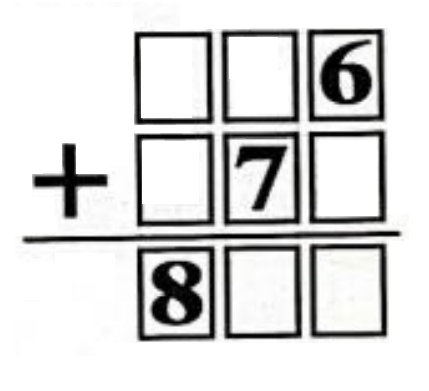
\includegraphics[width=0.3\textwidth]{./pics/Chapter_7/3.png}
    % \end{figure}
    \vspace{1cm}
    % 2023YCB初赛真题答案小中.pdf; 819
    % 改
}

\item {
    【数字谜】
    在右图的加法竖式中,6个汉字恰好代表6个连续的数字,那么,``花园探秘'' 所代表的四位数是\underline{\hbox to 20mm{}}.
    \zihao{3}
    \[
    \begin{array}{l@{\hspace{1em}} c@{\hspace{1em}} c@{\hspace{1em}} c@{\hspace{1em}} c@{\hspace{1em}}}
    & 第 & 3 & 3 & 届 \\
    + & 2 & 0 & 1 & 7 \\ 
    \hline
    & 花 & 园 & 探 & 秘 \\
    \end{array}
    \]
    % \begin{figure}[H] 
    %     \centering
    %     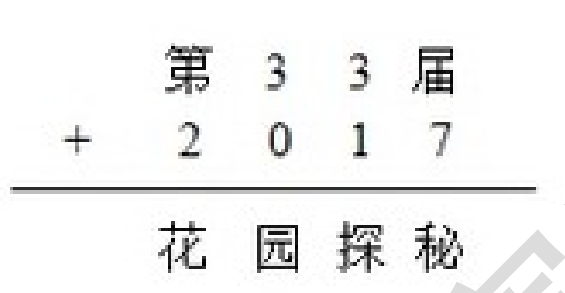
\includegraphics[width=0.4\textwidth]{./pics/Chapter_7/12.png}
    % \end{figure}
    % \vspace{1cm}
    % 2021; 8354
}

\item {
    【数字谜】
    在右面的乘法竖式中,相同的汉字代表相同的数字,不同的汉字代表不同的数字;那么,\myoverline{迎接夏天} 代表的四位数是\underline{\hbox to 20mm{}}.
    \zihao{3}
    \[
    \begin{array}{l@{\hspace{1em}}  c@{\hspace{1em}} c@{\hspace{1em}} c@{\hspace{1em}}}
    \quad & \quad & 迎 & 春 \\
    \times &\quad & 春 & 天 \\ 
    \hline
    \quad &\quad & 春 & 天 \\ 
    \quad & 晚 & 春 \\ 
    \hline
    迎& 接 & 夏 & 天 \\
    \end{array}
    \]
    % \begin{figure}[H] 
    %     \centering
    %     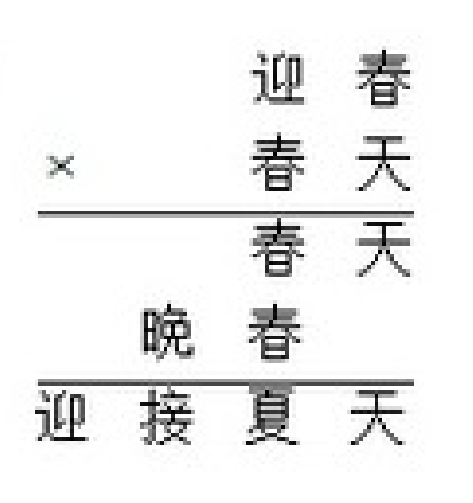
\includegraphics[width=0.4\textwidth]{./pics/Chapter_7/14.png}
    % \end{figure}
    \vspace{1cm}
    % 2021,迎春杯四年级真题.pdf; 1024
}


% \item {
%     【数字谜】
%     下列竖式中,相同汉字表示相同数字,不同汉字表示不同数字,且所有汉字对应的数字都不是 0,2,5.  ``空歌风度清'' 表示的五位数是\underline{\hbox to 20mm{}}.
%     \zihao{2}
%     \begin{figure}[H] 
%         \centering
%         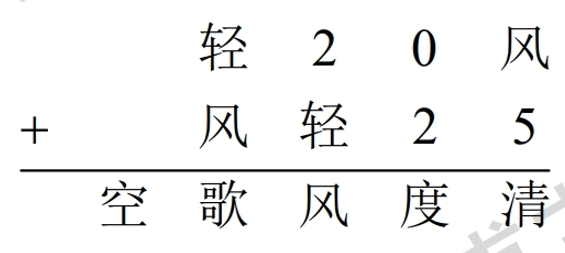
\includegraphics[width=0.4\textwidth]{./pics/Chapter_7/1.png}
%     \end{figure}
%     \vspace{1cm}
%     % 2025数学花园探秘笔试小中年级决赛C卷(B5试卷版).pdf;16934
% }

% \item {
%     $(20+2)\times 5 + 2025$ 
% }


% \item {
%     【乘法分配律】
%     $7\times 17 + 3\times 13\times 43 + 13\times 17$
%     \ifshowSolution
%         \fangsong\zihao{4}
%         \\
%         思路:2021;迎春杯四年级真题.pdf

%         正解: 2017
%     \else
%         \\ \\ \\
%     \fi
% }

% \item {
%     $(9\times 8\times 7 + 6 - 5)\times 4 + 3 -2 +1$
%     \ifshowSolution
%         \fangsong\zihao{4}
%         \\
%         思路: 迎春杯四年级2022-试卷.pdf

%         正解: 2022
%     \else
%         \\ \\ \\
%     \fi
% }